\documentclass[12pt, a4paper]{report}

\usepackage[a4paper,top=2cm,bottom=2cm,left=3cm,right=3cm,marginparwidth=1.75cm]{geometry}

\usepackage{graphicx}
\usepackage{amsmath}
\usepackage{longtable}
\usepackage{algorithm}
\usepackage{algpseudocode}
\usepackage{amssymb}
\usepackage[french]{babel}
\usepackage[utf8]{inputenc}
\usepackage[T1]{fontenc}
\usepackage[colorlinks=true, allcolors=blue]{hyperref}
\usepackage{float}
\usepackage{subcaption}
\usepackage{blindtext}
\usepackage{tabularx}
\usepackage{titlesec}
\usepackage{setspace}


\begin{document}
%%%%%%% HEAD %%%%%
\begin{titlepage}

	\newgeometry{right=2.5cm, left=2.5cm, top=2.5cm, bottom=2.5cm}
	
	\begin{center}
		
		{ \Huge \bfseries Cas d'étude :}
  
		\vspace{1cm}
  
        {\bfseries\Huge TP GREEN IT 2}
		
		
		\vspace*{1cm}

        \hfill

	    
		\Large \textbf{Filière : Systèmes informatiques pour le génie de la logistique industrielle et des services (SIGLIS)}\\

        \vspace{2cm}

       
  
  
        \begin{figure}[H]
        \centering
            
\includegraphics[width=10cm]{uppa.png}
        \end{figure}



        \end{center}

\vspace{3cm}


\begin{minipage}{0.4\textwidth}
\begin{flushleft} \large
\emph{Done by :}\\[0.5 cm]
ADIL \textsc{Nawfal}\\
COMBIER \textsc{Clement}\\

\end{flushleft}
\end{minipage}
\hfill
\begin{minipage}{0.5\textwidth}
\begin{flushright} \large
\emph{Sous la direction de :} \\[0.5 cm]
\textsc{Prof. NOUREDDINE \textsc{Adel}}\\

\end{flushright}
\end{minipage}

\vfill

% Bottom of the page
\begin{center}
{\large \ Année scolaire 2023/2024}
\end{center}
	
	\restoregeometry
	
\end{titlepage}

\newpage

%%%%%%%%%%%%%%%% Main part %%%%%%%%%%%%%%%%


\titleformat{\chapter}{\bfseries\centering\Huge}{10pt}

\titleformat*{\subsection}{\Large\bfseries}
\titleformat*{\subsubsection}{\large\bfseries}
\titleformat*{\paragraph}{\large\bfseries}
\titleformat*{\subparagraph}{\large\bfseries}

\setlength{\parindent}{3ex}

\doublespacing


\newpage

\fontsize{12}{12} \selectfont

%ne pas numéroter cette page
\thispagestyle{empty}
\newpage


\titleformat{\section}{\normalfont\bfseries\flushleft\Large}{\thesection.}{0.5em}{}

\titlespacing{\section}{12pc}{1.5ex plus .1ex minus .2ex}{1pc}

\setcounter{page}{0}

\newpage
\listoffigures

\newpage

\tableofcontents

\newpage

\chapter{\centering Introduction}

\subsection{Contexte du projet}
Pour ce second projet, nous souhaitons réaliser des modèles de puissance (Power Model) à travers l'utilisation PowerSpy, ainsi que de l'outil de benchmark CPUPowerBench (https://github.com/joular/cpupowerbench).
En green IT, la réalisation de Power model permettent de créer des analyses statistiques à l'aide de modèle de régression afin de pouvoir prédire la consomation d'un équipement.


\subsection{Objectif de l'étude}
Ic, nous travaillerons sur une RaspberryPI modèle 4 ainsi qu'un écran de la marque HP P22h G4. A travers deux expériences, nous utiliserons un Wattmètre PowerSpy ainsi que les outils du projet PowerJoular afin de relever la consommation pendant un benchmark de nos deux appareils.
Les outils de la suite Powerjoular utilisé ici seront :
\begin{itemize}
    \item PowerJoular : A des fins de relevés statistiques supplémentaires (Nous avons décidé d'utiliser cet outil de façon supplémentaire à la recherche à des fins purement statistique)
    \item CPUPowerBench : Afin de réaliser des benchmarks pour nos appareils.
    \item PowerSpiCLI : Notre environnement se basant sur Linux à travers la Raspberry PI, nous utilisons cette outil pour prendre les mesures faites par notre appareil PowerSpy pendant les benchmarks.
\end{itemize}

\chapter{\centering Fondements Théoriques \& Méthodologie Expérimentale}

\subsection{Méthodologie utilisée}
Pour avoir des dataseets statistiquement viable à la fin, nous allons suivre une méthodologie et un process claire et définie en amont afin de réaliser les expériences dans les meilleurs conditions possibles. Les expériences étant légèrement différente, nous avons développé deux processus distincts pour réaliser cette étude.
Voici notre méthodologie de base dans ce cas d'étude afin de répondre à la problématique de ce cas d'étude.
\begin{enumerate}
    \item Création de benchmark pour nos appareils
    \item Relevé de la consommation énergétique
    \item Création d'un modèle à partir de notre benchmark et de nos modèles
    \item Évaluation du modèle créé
\end{enumerate}

Voici la méthodologie ci-dessus sour forme de diagramme librement disponible sur GitHub : 
\begin{figure}[H]
    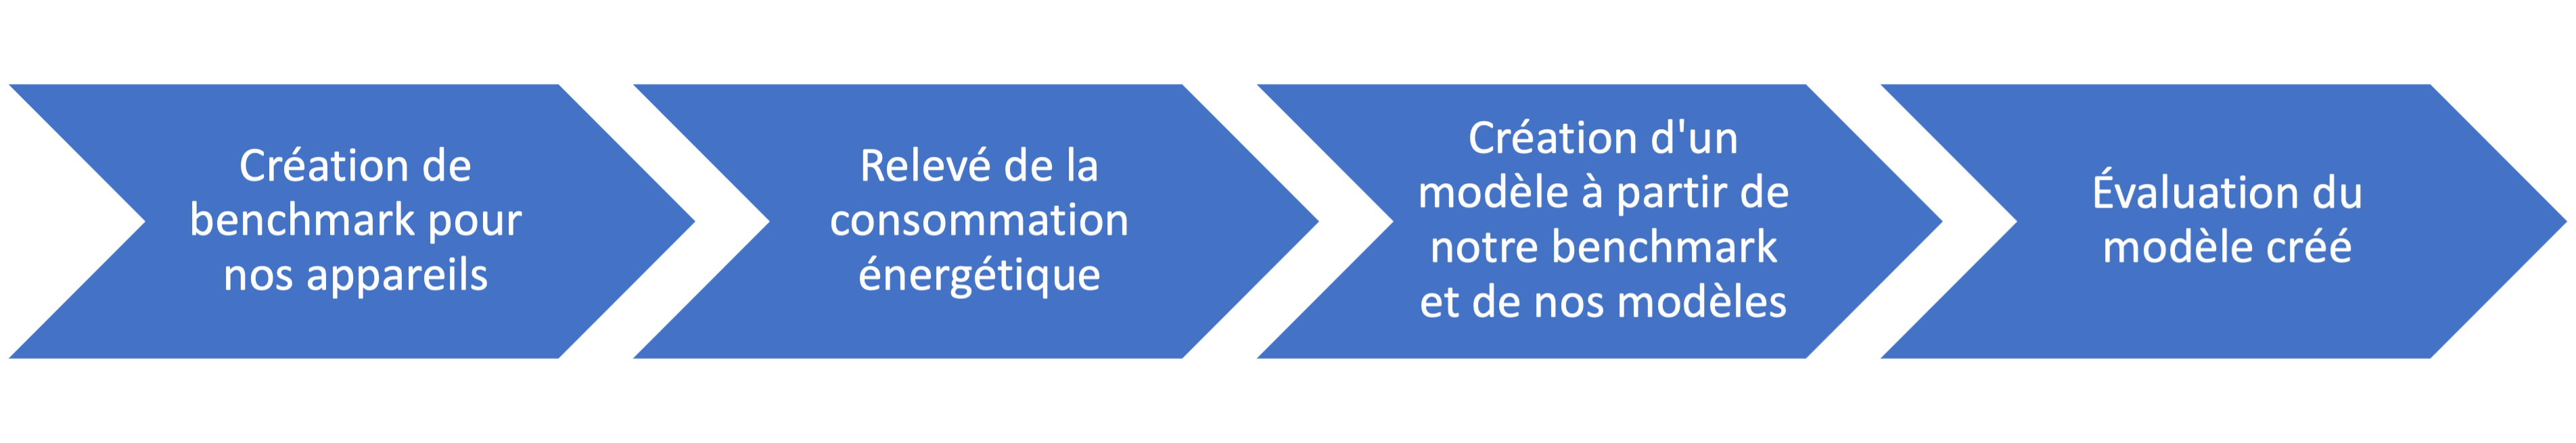
\includegraphics[width=1\linewidth]{res//process/processGlob.png}
    \caption{Méthodologie utilisée}
    \label{fig:méthodo}
\end{figure}

Maintenant, voyons plus en détail pour chacune des expérience (pour chaque appareil testé), comment nous allons nous y prendre, en incluant les outils utilisés, les étapes clefs, les résultats et l'attente finale.

\subsubsection{Étude Raspberry PI}
Pour l'étude sur la RaspberryPI, les étapes que nous avons suivi sont les suivantes :
\begin{enumerate}
    \item Télécharger et préparer les outils
    \item Tuer tous les processus non nécessaire en arrière plan
    \item Lancer l'analyse PowerSpy à l'aide de PowerSpyCLI
    \item Lancer le benchmark à l'aide de l'outil CPUPowerBench
    \item Enlever les périphériques de la RaspberryPI (écrans, souris, claviers, etc.)
    \item Après la fin du benchmark, récupérer les datasets
    \item Utiliser l'outil proposé par CPUPowerBench pour la réalisation de notre modèle à l'aide de nos trois datasets.
    \item Réalisation de l'étude statistique et évaluation du modèle
\end{enumerate}

Voici ce processus sous forme de graph :
\begin{figure}[H]
    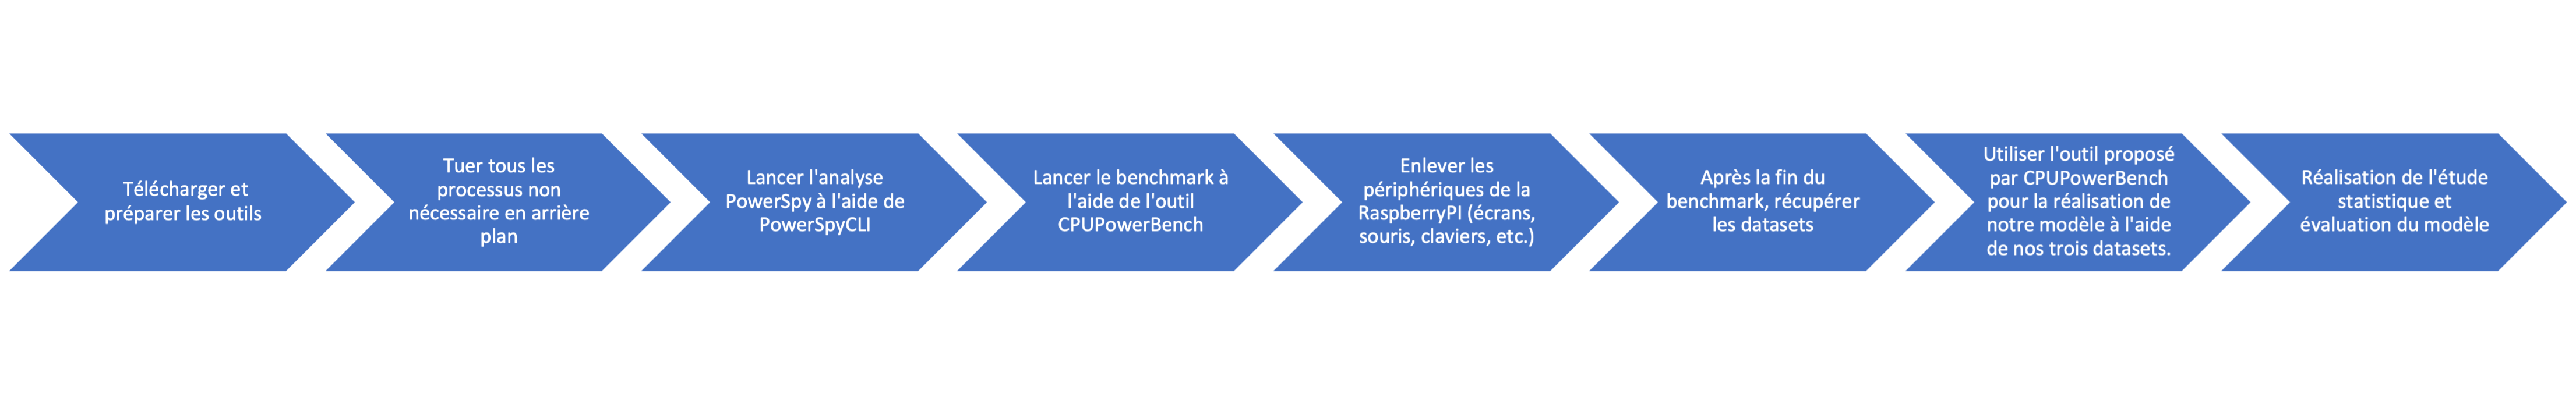
\includegraphics[width=1\linewidth]{res//process/ProcessusRPi.png}
    \caption{Processus de l'expérience #1 sur la RaspberryPi}
    \label{fig:experience-process_rpi}
\end{figure}

\subsubsection{Étude sur l'écran}
Un processus similaire à était utilisé poue l'étude de notre écran HP P22h G4. Nous avons fais la même étude en modifiant les paramètres de l'écran (luminoité, contraste, etc.) comme forme de benchmark. 

\chapter{\centering Résultats}

\subsubsection{Raspberry Pi}

\subsubsubsection{Régression Joular}
Pour cette première expérience sur la Raspberry Pi, nous avons pris les données fournis en fin d'expérience par la suite Joular pour effectuer notre analyse. Celle-ci contenait déjà une première régression linéaire faite en python.
Voci son résultat :
\begin{figure}[H]
    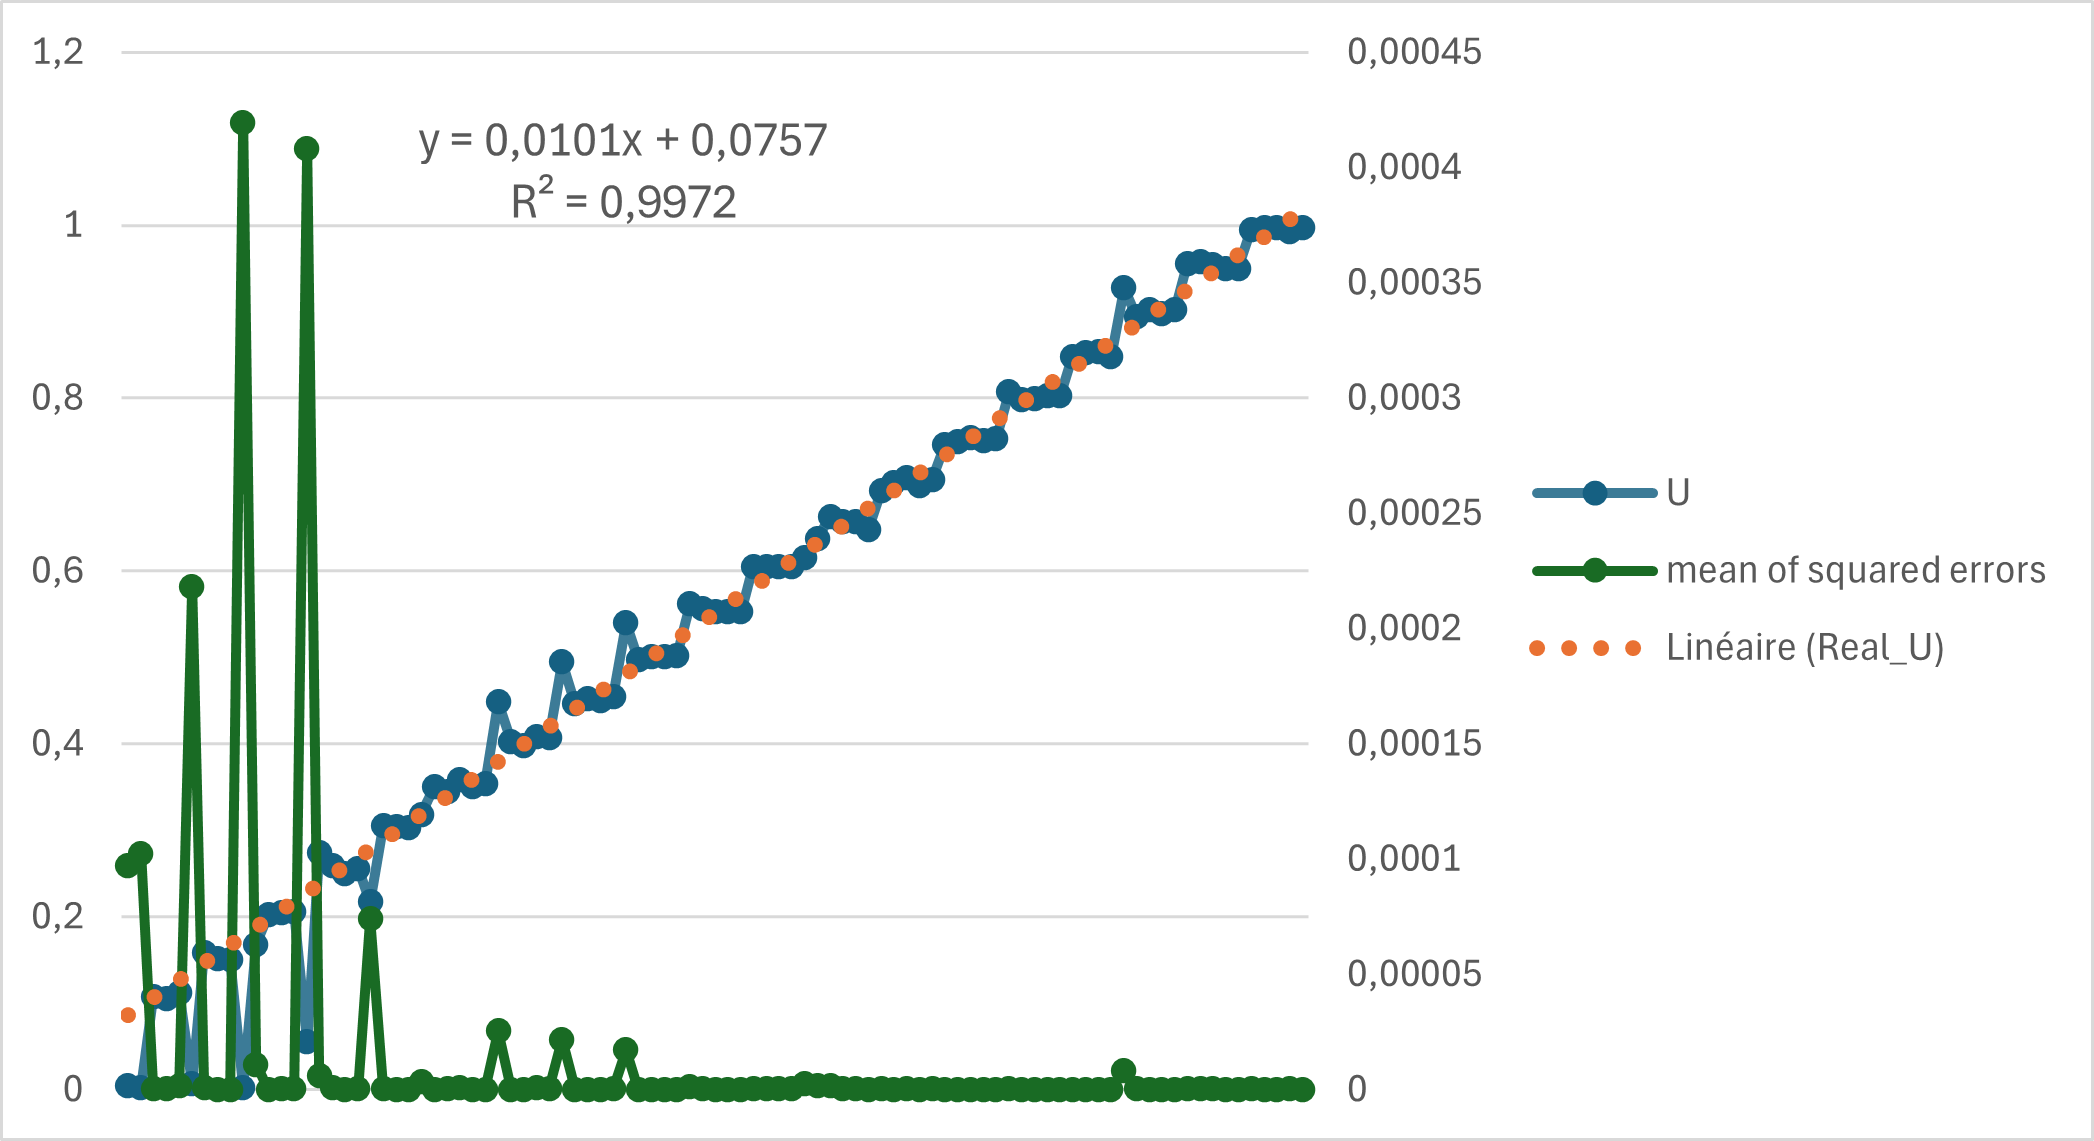
\includegraphics[width=1\linewidth]{res/graph/RPi/measure1.png}
    \caption{Régression Joular}
    \label{fig:reg_joular}
\end{figure}

comme nous pouvons le voir, le modèle de puissance suit bien une courbe de tendance linéaire. Notre score R² n'est pas muavais, à environ 99\% (R²=0,9972) et l'équation de notre courbe est la suivante : 
\begin{equation}
    y=0.0101x+0,0757
    \label{eq:rpi_joular}
\end{equation}
La courbe verte montre nos valeurs MSE qui tourne autour de 0 mis à part certains pics allant jusqu'à maximum 0.00045 ce qui reste très bas et donc très bon. Le modèle fournis représente donc bien la consommation de notre RaspberryPi et le modèle fit bien le cas d'étude.

Pour vérifier, nous avons décidé de faire la régression linéaire nous même sur Excel.

\subsubsubsection{Régression manuelle}
Cette régression a été faite sous Excel en utilisant les jeux de données de la première expérience. Voci le graphique en fin de modélisation.
\begin{figure}[H]
    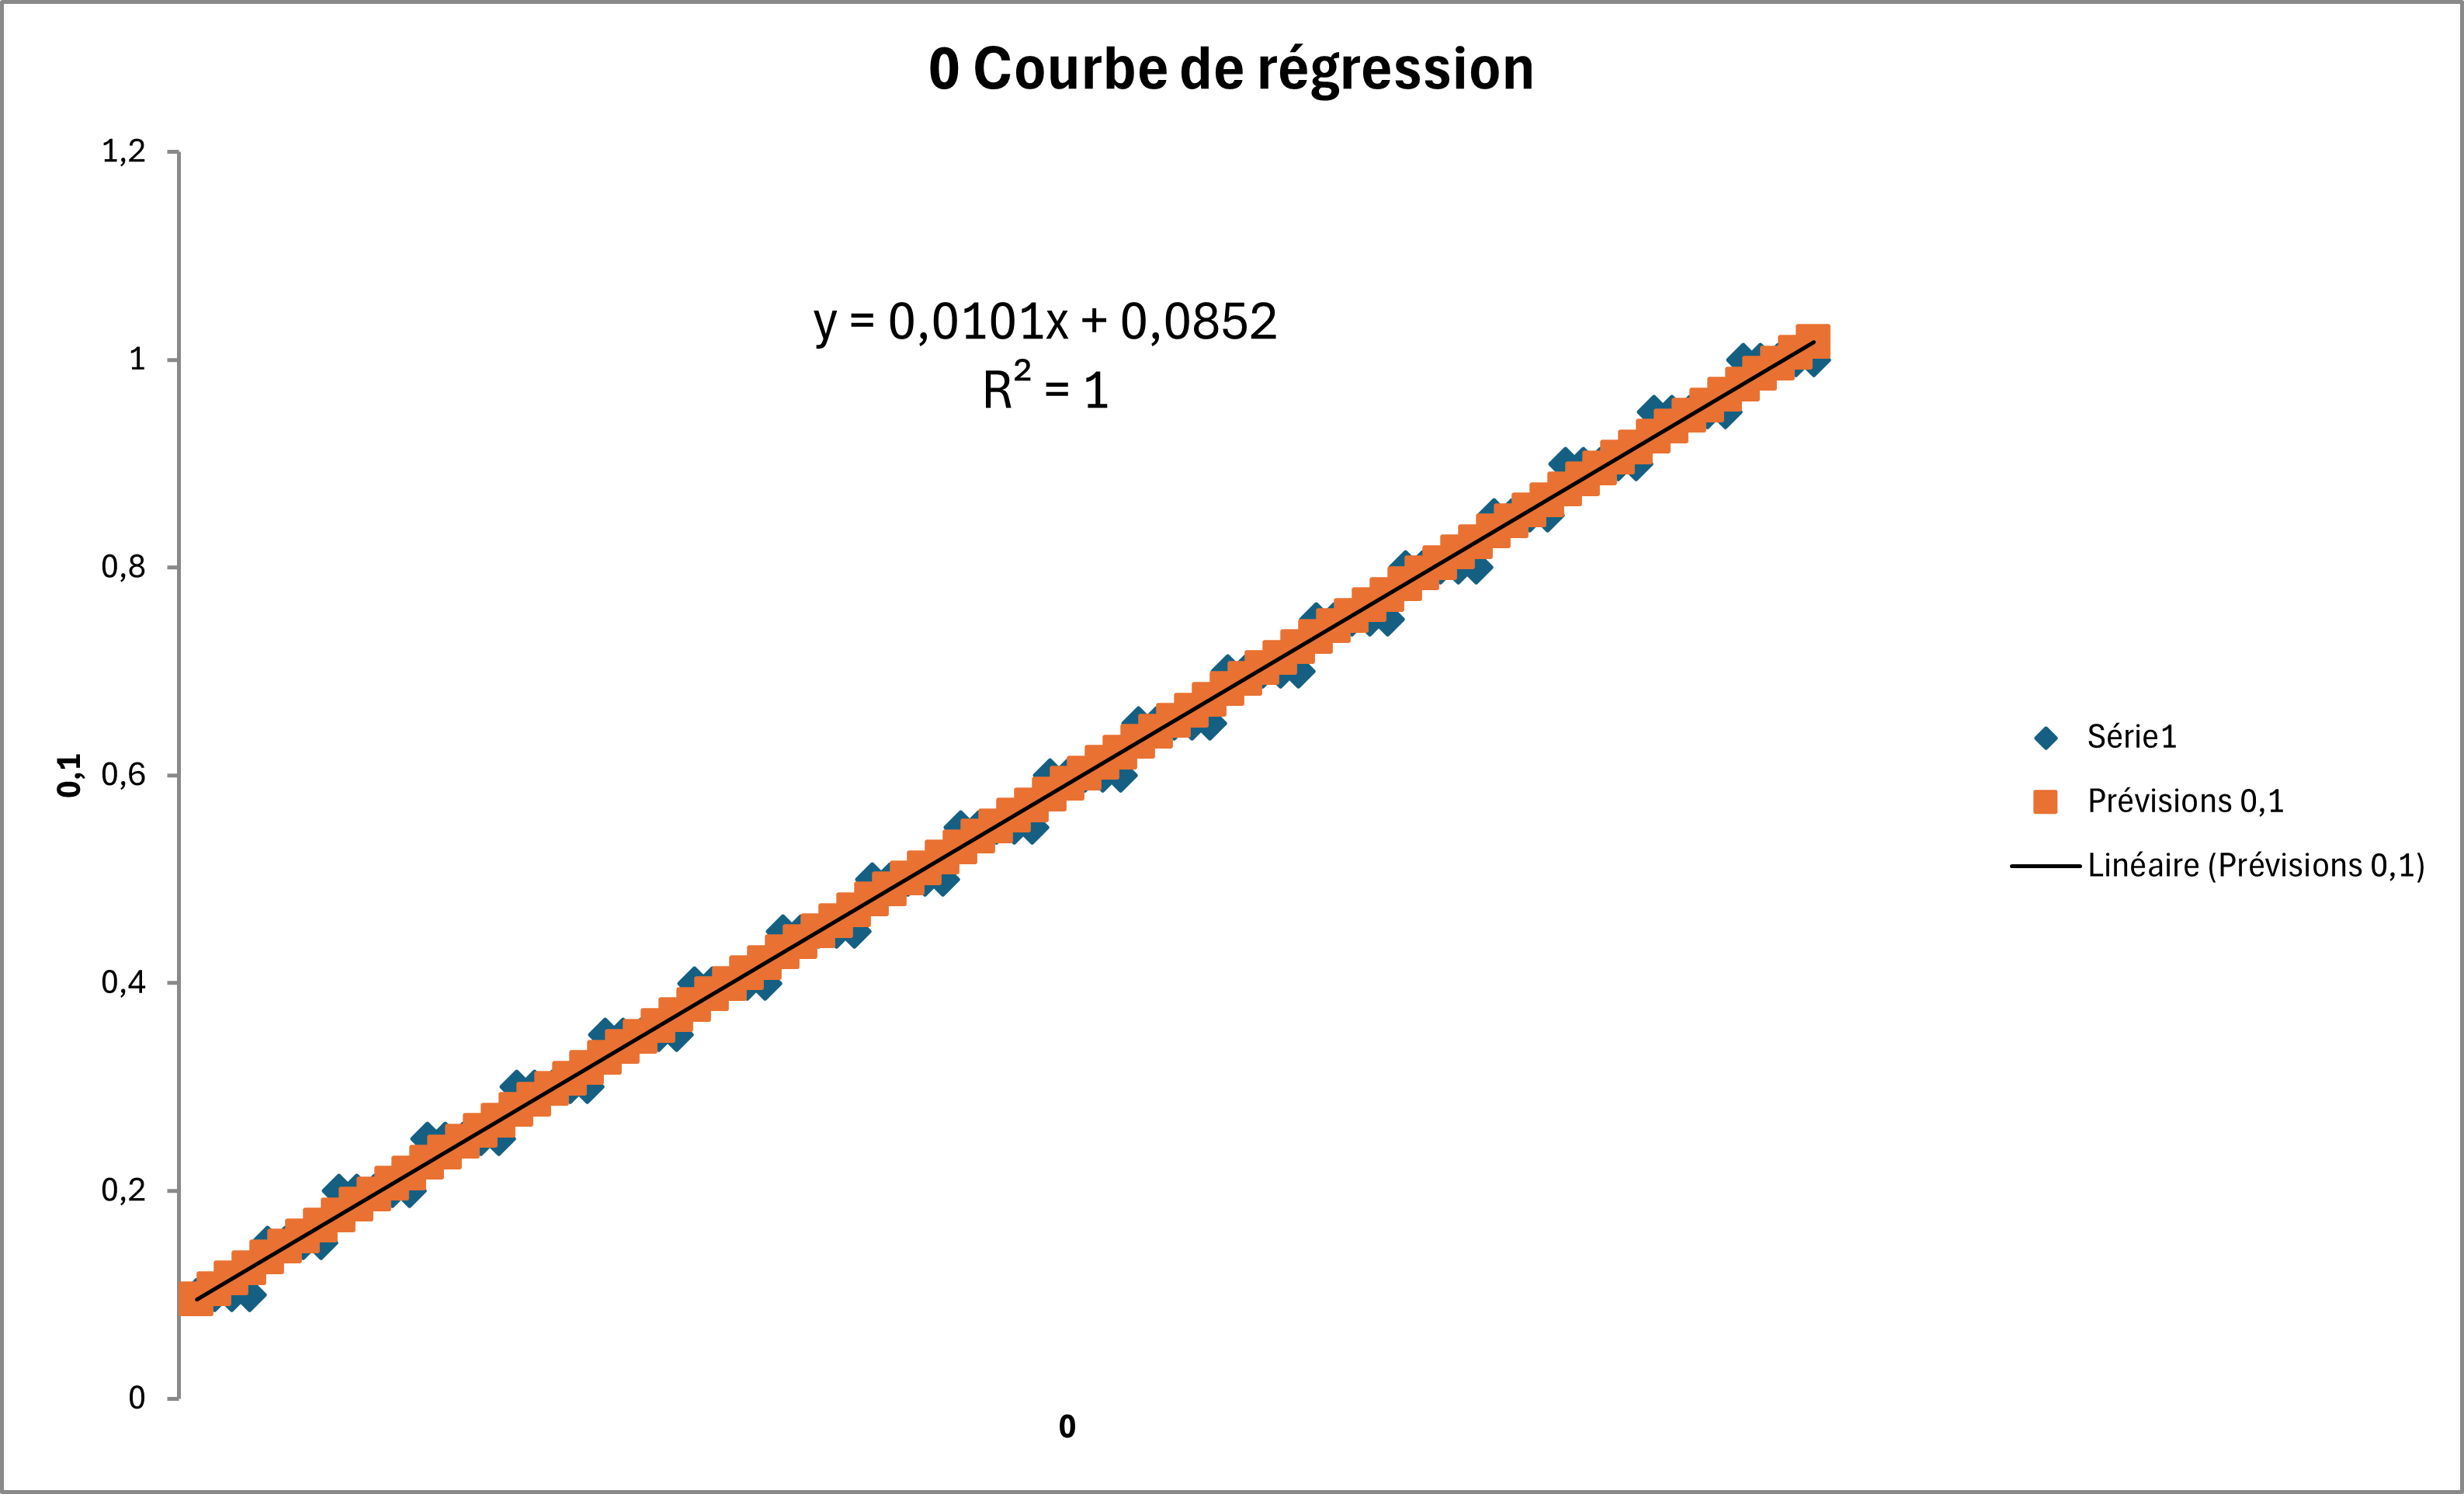
\includegraphics[width=1\linewidth]{res/graph/RPi/regman.png}
    \caption{Régression manuelle sur Excel}
    \label{fig:reg_man}
\end{figure}
Comme précédemment, nous retrouvons une tendance linéaire, collant bien avec la régression donné par Joular et suivant le même patterne et les mêmes ordres de grandeurs. 
L'équation ainsi que le R² sont quasiment semblable. Les résultats sont donc encourageants.

\subsubsection{Écran HP P22h G4}
Pour cette deuxième expérience, nous avons mené le même type d'expérience mais cette fois le benchmark était fait manuellement sur le moniteur (de la marque HP P22h G4) en modifiant manuellement les paramètres de ce dernier (luminosité, contraste, etc.) par intervalle régulier. Nous avons branché le WattMètre PowerSpy à l'alimentation de l'écran, et nous avons suivi quasiment le même procédé.
Voici le modèle et le résultat :

\begin{figure}[H]
    \includegraphics[width=1\linewidth]{res/graph/Ecran/Evolution de la puissance (luminosité).png}
    \caption{Evolution de la puissance (luminosité)}
    \label{fig:evolution-puis}
\end{figure}

On peut observer une augmentation de la puissance en fonction du temps de façon linéaire, qui est due à l'augmentation de la luminosité de façon périodique, les petits pics d'augmentation de puissance correspondent aux moments d'augmentation de luminosité. On peut donc constater une directe liaison entre la luminosité de l'écran et la consommation d'énergie.
Le modèle suit bien une fonction linéaire, et comme précédemment, le score R² est très satisfaisant (R²=0.9932) et l'équation de la courbe dde tendance linéaire suivant nos résultats :
\begin{equation}
    y=0.00746x+5.7349
    \label{eq:moniteur}
\end{equation}
Nous n'avons pas eu le temps malheureusement d'approfondir cette analyse.

\chapter{\centering Discussion}
Ces résultats permettent de montrer l'utilité du benchmarking et de créer des modèles de puissance (Power Model) dans le domaine du GreenIT.
Mais nous avons quelques points que nous devons éclairer et discuter pour expliquer l'état de cette étude.

\subsection{Fiabilité des outils de mesure utilisés}
Les autres outils ont déjà prouvé être efficace dans ce domaine, et la suite d'outils du projet Joular sont constamment amélioré et mis à jour (i.e. ce n'est pas un abandonware délaissé mai un projet activement développé!)

\subsection{Limitations de l'étude et pistes pour des recherches futures}
Pour l'instant, notre étude reste très simple ou nous avons beaucoup d'étapes manuelles. De plus, les RaspberryPi utilisées ont étaient utilisées par d'autres étudiants auparavant et incluaient déjà des applications, outils, etc. déjà utilisés. Une RaspberryPi avec un OS fraîchement installé pourrait donner de meilleurs relevés sur la consommation d'une RPi à travers d'un benchmark.
Par manque de temps est à cause de problème rencontré avec le matériel, nous n'avons pas eu la possibilité de pousser nos analyses et nos expérimentations avec la création d'autres modèles.

\chapter{\centering Conclusion}
La réalisation de benchmark sur différents appareils IT sont très utiles pour l'avancer et la démocratisation du domaine du Green IT.
Il est important de régulièrement testé nos appareils pour vérifier leur efficacité, leur consommation et potentiellement détecter les appareils qui ont des défauts majeurs qui font que nous perdons plus économiquement qu'ils nous en apportent.


\end{document}